\begin{frame}[fragile]{Tutorial: Custom two-site operators}

\begin{columns}

\begin{column}{5.5cm}

\begin{onlyenv}<1->
\begin{lstlisting}[language=JuliaLocal, style=julia, mathescape, basicstyle=\small]
CH = op("CRy", i1, i2; $\theta$=$\pi$/2)
\end{lstlisting}
\end{onlyenv}

\begin{onlyenv}<3->
~\\
\begin{lstlisting}[language=JuliaLocal, style=julia, mathescape, basicstyle=\small]
apply(CH, Zp1 * Zp2) ==
      Zp1 * Xp2
\end{lstlisting}
\end{onlyenv}

\end{column}

\begin{column}{4.5cm}

\begin{onlyenv}<1-1>
Controlled-Hadamard gate \\
CH = CRy($\theta$=$\pi$/2)
\end{onlyenv}

\begin{onlyenv}<2->
\vspace*{0.0cm}
\begin{center}
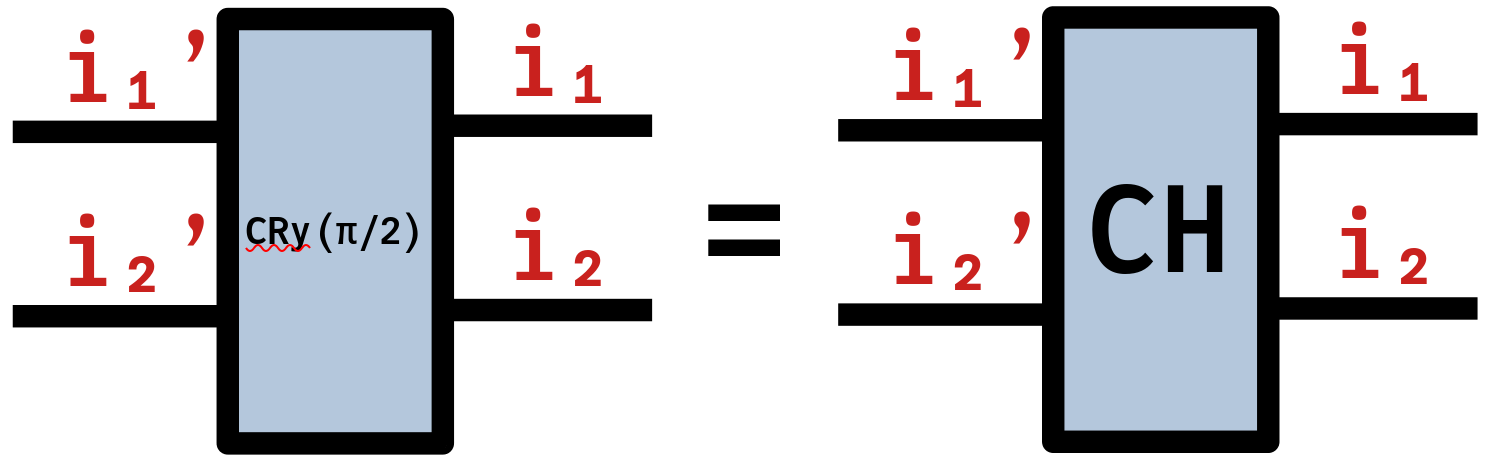
\includegraphics[width=1.0\textwidth]{
  slides/assets/CH12.png
}
\end{center}
\vspace*{0.0cm}
\end{onlyenv}

%% \begin{onlyenv}<3->
%% ~\\
%% \end{onlyenv}

\begin{onlyenv}<3-3>
~\\
CH|Z+Z+$\rangle$ = |Z+X+$\rangle$ \\
~\\
~\\
\end{onlyenv}

\begin{onlyenv}<4->
\vspace*{0.0cm}
\begin{center}
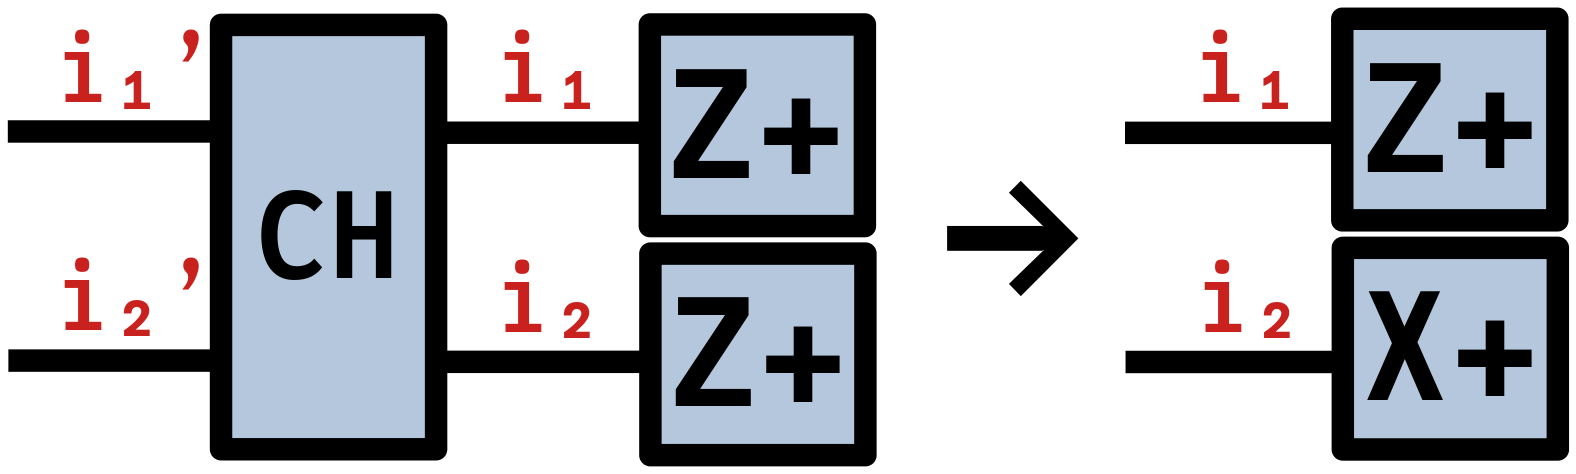
\includegraphics[width=1.0\textwidth]{
  slides/assets/CHZp1Zp2_to_Zp1Xp2.png
}
\end{center}
\vspace*{0.0cm}
\end{onlyenv}

\end{column}

\end{columns}

\end{frame}
